\documentclass[11pt,a4paper]{article}

\usepackage[utf8]{inputenc}

\usepackage[margin=2.5cm]{geometry}
\usepackage{amsmath,amssymb,amsthm}
\usepackage{booktabs,tabularx,array}
\usepackage{enumitem}
\usepackage{tikz}
\usetikzlibrary{arrows.meta,positioning}
\usepackage[hidelinks]{hyperref}
\usepackage{xurl}

\newtheorem{proposition}{Proposition}
\newcommand{\code}[1]{\path{#1}}
\urlstyle{tt}
\newcommand{\cmd}[1]{\texttt{\detokenize{#1}}}
\newcolumntype{Y}{>{\raggedright\arraybackslash}X}

\title{CE390 $d$-first search for $A^3+B^3+C^3=390$:\\ rationale and modus operandi}
\author{Jamal Agbanwa}
\date{29 October 2026}

\begin{document}
\maketitle

\begin{abstract}
The CE390 scripts turn the search for integer solutions of $A^3+B^3+C^3=390$ into a finite,
exactly certified sweep over rational slopes $d=p/q$. For each slope, a binary cubic Thue
equation is solved completely for every scale $1\le|g|\le10^{100}$. Slopes are enumerated in
shells of increasing height, and the campaign is sized for the 1{,}800 core-hours allocated to it out of a
2{,}000-hour Charity Engine grant (200 hours go to other projects). This note gives the mathematical reduction, the proved filters, the
exact meaning of a completed range, the software pipeline, the validation evidence, the
operating procedure and the limits of the method.
\end{abstract}

\tableofcontents

%--------------------------------------------------------------------
\section{Purpose and target}

The search works in a \emph{half-integer chart}. It looks for a rational $d$, an integer
$n\equiv1\pmod 3$, and half-integers $x=X/2$, $y=Y/2$ with $X,Y$ odd and $Y>0$, such that
\begin{equation}\label{eq:target}
  y^2=(x+6n)^2+\frac{36n^3-65}{x},\qquad
  36n^3-65=-2\,d\,x^2\bigl(y-(x+6n)\bigr).
\end{equation}
Any such point yields integers $A=-x+y$, $B=-x-y$, $C=2x+6n$ with $A^3+B^3+C^3=390$.
Both signs of $n$ and $X$ are searched, and every accepted value is checked with exact
integer arithmetic.

The code lives in the repository
\url{https://github.com/JAgbanwa/SomethingNew/tree/main/390%20/Scripts%20for%20large-scale%20computations%20}.
This note describes the revision reviewed on 29 October 2026.

%--------------------------------------------------------------------
\section{Mathematical rationale}

Every integer representation of $390$ corresponds to an integer solution of one binary
cubic Thue equation in $(n,g)$, indexed by a rational $d$. Enumerating $d$ by height and
solving each equation completely is therefore a search over all representations, ordered
by the height of $d$. Throughout, $m$ denotes the parameter with $k=6m$. Production uses
$m=65$ ($k=390$); $m=1$ ($k=6$) is used only as a detection test.

\subsection{Cube-sum identity}
With $A=-x+y$, $B=-x-y$, $C=2x+6n$, direct expansion gives
\begin{equation}
  A^3+B^3+C^3-6m=-6x\left(y^2-(x+6n)^2-\frac{36n^3-m}{x}\right).
\end{equation}
So a point of \eqref{eq:target} is exactly a representation of $6m$. When $X$ and $Y$ are
odd, $A=(Y-X)/2$, $B=-(X+Y)/2$ and $C=X+6n$ are integers.

\subsection{Pair sums and the closed form of $d$}
Let $u=A+B=-2x$, $v=B+C$, $w=C+A$. Then $u+v+w=12n$, and from
$(A+B+C)^3-(A^3+B^3+C^3)=3(A+B)(B+C)(C+A)$,
\begin{equation}
  uvw=2(36n^3-m).
\end{equation}
Since $y\ge0$ forces $A\ge B$, the slope simplifies to a ratio of pair sums:
\begin{equation}
  d=-\frac{y+x+6n}{2x}=\frac{A+C}{A+B}=\frac{w}{u}.
\end{equation}
Write $d=p/q$ in lowest terms with $q>0$. Then $u=qg$ and $w=pg$ for an integer $g$; that
is, $g=\pm\gcd(A+B,\,A+C)$.

\subsection{The Thue equation}
Substituting $v=12n-(p+q)g$ into $uvw=2(36n^3-m)$ gives, for each $d$,
\begin{equation}\label{eq:thue}
  F_d(n,g)=72n^3-12pq\,n\,g^2+pq(p+q)\,g^3=2m=130.
\end{equation}

\begin{proposition}
Every integer solution $(n,g)$ of \eqref{eq:thue} with $qg$ odd and $Y=(2p+q)g-12n>0$ gives
a half-chart point via $x=-qg/2$, $y=Y/2$; conversely every half-chart point arises this way.
Moreover, identically in $p,q,g,n$,
\[
  A^3+B^3+C^3-390=3\bigl(F_d(n,g)-130\bigr).
\]
\end{proposition}

The identity was checked symbolically (SymPy) as part of this review. Solutions with $Y<0$
belong to the conjugate slope $v/u$, and solutions with $g$ even belong to the integer
chart. The worker counts both kinds but does not report them.

\subsection{Congruences and completeness of the chart}
\begin{itemize}[leftmargin=*]
  \item \textbf{$n$ is an integer.} Since $3\nmid65$, we have $6m\equiv3$ or $6\pmod 9$; as cubes
  are $0,\pm1\pmod 9$, this forces $A\equiv B\equiv C\pmod3$, so $3\mid A+B+C$. Parity makes
  $A+B+C$ even, so $6\mid A+B+C$ and $n=(A+B+C)/6\in\mathbb{Z}$.
  \item \textbf{$n\equiv1\pmod3$.} For $390\equiv3\pmod 9$, each component is $\equiv1\pmod3$,
  and $t^3\equiv3t-2\pmod{27}$ for such $t$ gives $390\equiv18n-6\pmod{27}$, hence $n\equiv1\pmod3$.
  \item \textbf{No representation is lost.} The number of odd cubes is even and cannot be zero
  (since $8\nmid390$), so exactly one component is even. Pairing it with either odd component
  gives an odd pair sum $u$. Every representation therefore has two half-chart points, and
  both signs of $n$ and $X$ are searched.
\end{itemize}

\subsection{Solving one equation completely up to $|g|\le G$}
The cubic $f(t)=F_d(t,1)=72t^3-12pq\,t+pq(p+q)$ has discriminant
$-15552(pq)^2(9p^2-14pq+9q^2)<0$, so it has one real root $\alpha$ and complex roots
$\beta,\bar\beta$ with $\eta^2=(\operatorname{Im}\beta)^2=\tfrac34\alpha^2-\tfrac{pq}{6}>0$.
Any solution satisfies
\begin{equation}
  \left|\frac ng-\alpha\right|\le\frac{|T|}{72\,\eta^2\,|g|^3},\qquad T=2m=130.
\end{equation}
\begin{itemize}[leftmargin=*]
  \item \textbf{Large $g$.} For $|g|>g_0=|T|/(36\eta^2)$ the bound is below $1/(2g^2)$, so by
  Legendre's theorem $n/g$ is a continued-fraction convergent of $\alpha$. As $130$ is
  cube-free, $\gcd(n,g)=1$. The worker brackets $\alpha$ by exact integer sign tests, accepts a
  partial quotient only when both bracket ends agree, and doubles precision on disagreement.
  It stops only once the next denominator exceeds $G=10^{100}$, and raises an error rather than
  certifying if a precision cap is reached.
  \item \textbf{Small $g$.} For $1\le|g|\le g_0$, all integer roots $n$ are found by exact binary
  search on the monotone pieces of the cubic. Usually $g_0\in\{0,1\}$; it is large only near
  $d=1$ (about $1{,}640$ at $d=1$).
  \item \textbf{Rational $\alpha$.} This occurs only at $d=-1$ (excluded by the filters) and is
  detected and bounded separately.
\end{itemize}
By Thue's theorem each $d$ has finitely many solutions. For an unbounded certificate of a
single $d$, \code{tools/certify_d.gp} calls PARI's \code{thue()} with unconditional bounds.

%--------------------------------------------------------------------
\section{Filters: which $d$ are worth solving}

Every filter in Table~\ref{tab:filters} is a proved necessary condition, so excluding a $d$
never loses a solution. Up to height $120$, the current filters leave $517$ admissible
fractions, down from $789$ under the earlier filter, and none of the seven known $k=6$
certificates is excluded.

\begin{table}[h]
\centering\small
\caption{Necessary conditions on $d=p/q$, $q>0$, for a half-chart point.}\label{tab:filters}
\begin{tabularx}{\textwidth}{>{\raggedright\arraybackslash}p{0.42\textwidth}Y}
\toprule
Condition & Reason \\
\midrule
$q$ odd, $g$ odd & $u=qg=-X$ must be odd \\
$3\nmid pqg$ and $p\equiv q\pmod3$ & $A\equiv B\equiv C\equiv\varepsilon\pmod 3$, so $u\equiv w\equiv2\varepsilon\not\equiv0$ \\
$p(p+q)\equiv2\pmod4$ & \eqref{eq:thue} mod 4 with $q,g$ odd; equivalently $p\equiv2\pmod 4$ ($p$ even) or $p\equiv q\pmod4$ ($p$ odd) \\
$25\nmid pq$ and $169\nmid pq$ & for $\ell\mid65$: $v_\ell(36n^3-65)\le v_\ell(65)$ \\
every prime $\ell\equiv1\pmod3$, $\ell\nmid65$, dividing $p$ or $q$ admits $36t^3\equiv65\pmod\ell$ & $u,w$ divide $2(36n^3-65)$ \\
\bottomrule
\end{tabularx}
\end{table}

The last condition generalises the repository's older 733-prime $q$-sieve to all primes and
to both numerator and denominator. Signed numerators are reduced to non-negative residues
before the mod-4 test. The native worker, the Python reference \code{dfirst_common.admissible}
and the PARI helper implement the filters independently, and the tests check that they agree
shell by shell.

%--------------------------------------------------------------------
\section{Search geometry and what it can reach}

The search runs over two axes: the height $H(d)=\max(|p|,q)$, swept in shells up to about
$800{,}000$, and the scale $|g|$, covered completely up to $10^{100}$ for each $d$. A
solution is found exactly when its own $d$ and $g$ lie inside both bounds.

\subsection{Height shells}
Shell $H$ contains the $4H-1$ raw pairs $(p,q)$ with $\max(|p|,q)=H$, so cumulative work is
$P(H)=2H^2+H$. Tasks are contiguous, disjoint, half-open shell ranges $[a,b)$; completing
shells $1,\dots,H$ settles every $d$ of height at most $H$.

\subsection{What a completed range proves}
For each returned range $[a,b)$, \code{collect_d.py} records the claim:
\begin{quote}
No $d=p/q$ with $a\le\max(|p|,q)<b$ has a point with $n\equiv1\pmod3$, $x=X/2$, $y=Y/2$
($X,Y$ odd, $Y>0$) and $1\le|g|\le10^{100}$, other than the listed, exactly verified hits.
\end{quote}
This is a bounded statement: it covers the recorded heights and the $g$ bound, not all
coordinates.

\subsection{Which solutions fall inside}
Since $u=qg$ and $w=pg$, we have $H(d)=\max(|A+B|,|A+C|)/|g|$, and \eqref{eq:thue} gives
$n\approx H(d)\,g$. Hence every cube component is roughly $H(d)\times|g|$.

\begin{table}[h]
\centering\small
\caption{Reach of the campaign by type of solution.}
\begin{tabularx}{\textwidth}{>{\raggedright\arraybackslash}p{0.3\textwidth}>{\raggedright\arraybackslash}p{0.22\textwidth}Y}
\toprule
Kind of solution & Coordinate size & Reached? \\
\midrule
Small $g$ & $\approx H(d)\lesssim10^6$ & Yes, but already covered by earlier direct searches (about $10^{16}$--$10^{17}$) \\
Large $g$, small $H(d)$ & $\approx H(d)\,g$, up to about $10^{106}$ & Yes; this is where new ground lies \\
Small $g$, coordinates $>10^{17}$ & needs $H(d)>10^{17}$ & No; height grows like the square root of compute \\
\bottomrule
\end{tabularx}
\end{table}

A new solution must therefore have coordinates above about $10^{17}$ with $|g|\gtrsim10^{11}$,
meaning two pair sums share a very large common factor. All seven known $k=6$ points have
$g=\pm1$. The campaign is best understood as a complete check of the large-$g$, small-height
region, which no coordinate-box search can reach.

\subsection{Relation to the old coordinate rectangle}
The earlier rectangle ($|n|\le10^{45}$, $|x|\ge10^{54}$) requires $q\ge1.7\times10^8$ for
$x>0$ and $q\approx5.6\times10^{25}$ for $x<0$, both far beyond any affordable height. The
$d$-first search explores a different region; it does not exhaust the old box.

%--------------------------------------------------------------------
\section{Software architecture}

Six components turn a budget into certified coverage (Figure~\ref{fig:arch}). Only the
native worker does mathematics at scale; every other stage plans, checkpoints or re-checks.

\begin{figure}[h]
\centering
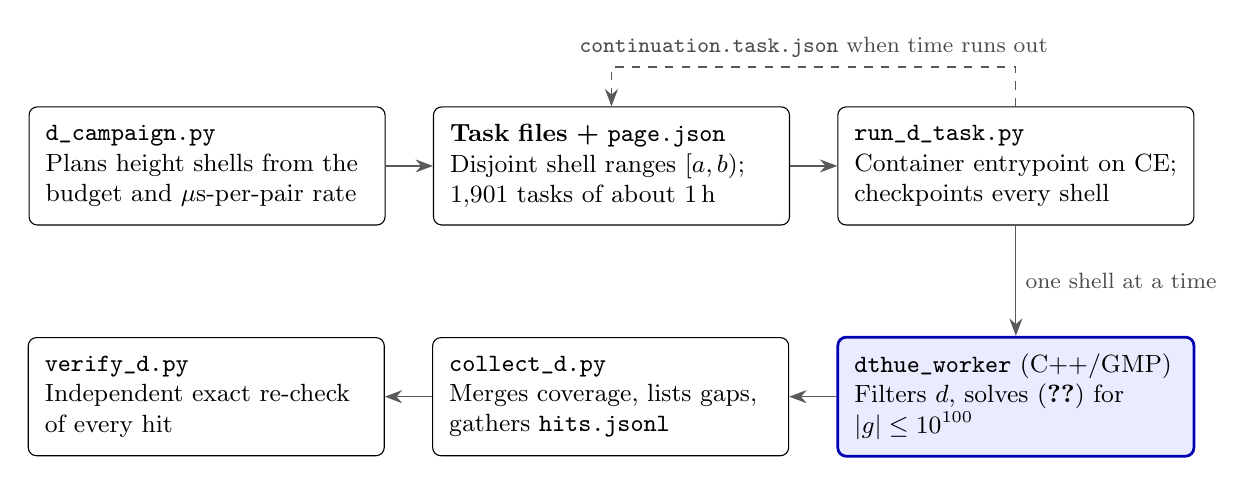
\begin{tikzpicture}[
  box/.style={draw, rounded corners=3pt, align=left, text width=4.1cm, minimum height=1.5cm, inner sep=6pt, font=\small},
  main/.style={box, draw=blue!70!black, fill=blue!8, line width=1pt},
  arr/.style={-{Stealth[length=2.2mm]}, gray!70!black},
  node distance=0.7cm and 0.6cm]
\node[box] (plan) {\textbf{\code{d_campaign.py}}\\Plans height shells from the budget and $\mu$s-per-pair rate};
\node[box, right=of plan] (tasks) {\textbf{Task files + \code{page.json}}\\Disjoint shell ranges $[a,b)$; 1{,}901 tasks of about 1\,h};
\node[box, right=of tasks] (run) {\textbf{\code{run_d_task.py}}\\Container entrypoint on CE; checkpoints every shell};
\node[main, below=1.4cm of run] (work) {\textbf{\code{dthue_worker}} (C++/GMP)\\Filters $d$, solves \eqref{eq:thue} for $|g|\le10^{100}$};
\node[box, left=of work] (coll) {\textbf{\code{collect_d.py}}\\Merges coverage, lists gaps, gathers \code{hits.jsonl}};
\node[box, left=of coll] (ver) {\textbf{\code{verify_d.py}}\\Independent exact re-check of every hit};
\draw[arr] (plan) -- (tasks);
\draw[arr] (tasks) -- (run);
\draw[arr] (run) -- node[right, font=\footnotesize, gray!60!black]{one shell at a time} (work);
\draw[arr] (work) -- (coll);
\draw[arr] (coll) -- (ver);
\draw[arr, dashed] (run.north) -- ++(0,0.5) -| node[pos=0.25, above, font=\footnotesize, gray!60!black]{\code{continuation.task.json} when time runs out} (tasks.north);
\end{tikzpicture}
\caption{The CE390 pipeline.}\label{fig:arch}
\end{figure}

A task that runs out of time returns a continuation for the remaining shells, which is
resubmitted as a new, separately charged job. Locally, \code{run_d_campaign.py} drives the
same runner serially under a durable \code{budget.json} ledger. \code{dfirst_common.py}
contains the independent Python filter and verifier, and \code{tools/certify_d.gp} gives
unbounded PARI certificates for single $d$. The Dockerfile builds and tests the workers in
one stage, then ships them with the Python scripts on \code{debian:bookworm-slim}.

%--------------------------------------------------------------------
\section{Validation evidence}

The pipeline builds cleanly, passes all 249 tests, recovers known $k=6$ solutions and
matches PARI on $1{,}934$ Thue equations. The first three rows of Table~\ref{tab:val} were
re-run independently on 29 October 2026; the remainder are recorded in the repository.

\begin{table}[h]
\centering\small
\caption{Validation summary.}\label{tab:val}
\begin{tabularx}{\textwidth}{>{\raggedright\arraybackslash}p{0.24\textwidth}Y>{\raggedright\arraybackslash}p{0.26\textwidth}}
\toprule
Check & Result & Source \\
\midrule
Checksums, build, tests & \code{SHA256SUMS} match; three GMP workers compile without warnings; 249 tests pass & re-run \\
Cube-sum reduction & $A^3+B^3+C^3-390=3(F_d-130)$ identically & re-run (SymPy) \\
$k=6$, heights $1$--$120$ & 3 hits, exactly verified, e.g.\ $65^3+(-58)^3+(-43)^3=6$ & re-run \\
$k=6$, heights $1$--$449$ & exactly $d=1,\ 22/7,\ -22/101,\ 1/181,\ 181,\ 7/439,\ 439/7$ & \code{validation/dfirst} \\
PARI cross-check & identical solution sets on 1{,}934 equations; 679 solutions, 10 beyond $g_0$ & \code{tools/pari_crosscheck.gp} \\
Brute force, planted & agreement for $|g|\le120$ and $\le3000$ near $d=1$; planted $g\ge10^4$ recovered as convergents & \code{tests/test_dfirst.py} \\
Filter agreement & native and Python admissible counts equal per shell & test suite \\
Restart lifecycle & interrupted tasks resume; continuations refuse a different binary & test suite \\
$k=390$, $H\le20{,}000$ & no point; no Thue solution at all ($14{,}168{,}321$ admissible $d$, earlier filter) & \code{validation/dfirst} \\
$k=390$, $H\le120$, unbounded & no point (PARI unconditional \code{thue()}) & \code{validation/dfirst} \\
\bottomrule
\end{tabularx}
\end{table}

\subsection{Measured throughput}
On one 2.8\,GHz Xeon core, the current worker's cost per raw pair fell with height
(Table~\ref{tab:speed}). All values are below the $4.5\,\mu$s planning rate, so the default
plan is conservative on this hardware. Volunteer Charity Engine hosts will differ, so these
figures justify a pilot, not a final rate.

\begin{table}[h]
\centering\small
\caption{Measured worker throughput, 29 October 2026.}\label{tab:speed}
\begin{tabular}{lrrr}
\toprule
Height slice & Raw pairs & Wall time (s) & $\mu$s per pair \\
\midrule
$1{,}000$--$1{,}399$ & $1{,}918{,}800$ & $6.5$ & $3.4$ \\
$100{,}000$--$100{,}399$ & $160{,}318{,}800$ & $386.6$ & $2.4$ \\
$790{,}000$--$790{,}039$ & $126{,}403{,}080$ & $173.0$ & $1.4$ \\
\bottomrule
\end{tabular}
\end{table}

%--------------------------------------------------------------------
\section{Budget and Charity Engine procedure}

Of the $2{,}000$ hours granted on Charity Engine, $1{,}800$ are allocated to this project and
$200$ to other projects. The default plan spends an estimated $1{,}600$ core-hours to reach
height $799{,}999$ in $1{,}901$ one-hour tasks, under the hard $1{,}800$-hour project ceiling.
The other $200$ project hours are headroom for pilots, retries and continuations; the $200$
hours for other projects are never drawn on. Estimated work is
\begin{equation}
  \text{core-hours}=\frac{(2H^2+H)\times(\mu\text{s per pair})}{3.6\times10^{9}}.
\end{equation}
At $4.5\,\mu$s this gives $25$ hours at $H=10^5$, $625$ at $5\times10^5$ and $1{,}600$ at
$799{,}999$. Because height grows as the square root of hours, a measured rate of
$2.5\,\mu$s would raise the reachable height to about $1.07\times10^6$.

\subsection{Operating steps}
\begin{enumerate}[leftmargin=*]
  \item \textbf{Build and test the image.} Run \cmd{sha256sum --check SHA256SUMS},
  \cmd{make -j2}, \cmd{make test}, then rebuild the container from this revision. An older
  published image does not pick up the current filter or entrypoint.
  \item \textbf{Pilot on Charity Engine.} Generate a few tasks at low, middle and high heights
  and run them on CE hosts. Compute the rate as $10^6\times\text{elapsed seconds}/\text{pairs}$
  from each returned status.
  \item \textbf{Generate the campaign.} Run \code{d_campaign.py} with the measured
  \code{--us-per-pair}, \cmd{--budget-core-hours 1800}, \cmd{--planned-core-hours 1600},
  \cmd{--g-max-digits 100}. This writes task files and \code{page.json} only.
  \item \textbf{Submit tasks.} Stage each as \code{/local/input/task.json}; the container runs
  \code{run_d_task.py} and writes to \code{/local/output}. Each task has a $3{,}600$\,s internal
  budget, historically within a two-hour provider allowance.
  \item \textbf{Handle continuations.} A task that runs out of time checkpoints after each
  completed shell and writes \code{continuation.task.json}; resubmit it as a new, charged job.
  Continuations pin the worker and Python hashes.
  \item \textbf{Account centrally.} Before each submission, reserve its maximum possible
  provider charge. Record job ID, task or continuation ID, cores, time allowance, status and
  actual charge. Never submit a job whose maximum charge exceeds the remainder.
  \item \textbf{Collect and verify.} Run \code{collect_d.py} to merge coverage, list gaps and
  gather hits, then \cmd{verify_d.py hits.jsonl --m 65} for an independent exact re-check.
\end{enumerate}

\subsection{Local ledger versus remote jobs}
\code{run_d_campaign.py} enforces the ceiling with a durable \code{budget.json}: it reserves
each attempt's full duration before launch, charges elapsed time afterwards and blocks
restart after an unreconciled crash. It does not see Charity Engine jobs, so step~6 is a manual
responsibility. A second results directory creates a second ledger; it does not add hours.

%--------------------------------------------------------------------
\section{Limits, expected outcomes and recommendations}

The guaranteed result of the full campaign is a certified exclusion: no $k=390$
representation with $H(d)$ up to about $800{,}000$ (higher after recalibration) and
$1\le|g|\le10^{100}$, apart from any verified hits. A discovery is possible only if a solution
has a large common factor $g$ between two pair sums. This region is valid but narrow, and a
discovery should not be expected by default.

\subsection{Limits}
\begin{itemize}[leftmargin=*]
  \item \textbf{Height is the binding constraint.} Cost grows as $H^2$; doubling the reachable
  height needs four times the hours.
  \item \textbf{Generic large solutions are out of reach.} A solution with small $g$ and
  coordinates above about $10^{17}$ needs $H(d)>10^{17}$.
  \item \textbf{The $g$ bound is finite.} Each $d$ is settled only for $|g|\le10^{100}$.
  Unbounded certificates come from PARI \code{thue()}, practical so far only for $H\le120$.
  \item \textbf{Throughput is unconfirmed on Charity Engine.} All measured rates come from
  shared cloud cores.
  \item \textbf{Remote accounting is manual.} The local ledger does not bound CE charges.
\end{itemize}

\subsection{Recommendations}
\begin{enumerate}[leftmargin=*]
  \item \textbf{Recalibrate before the full run.} Pilot on CE across low, middle and high
  heights and regenerate with the measured \code{--us-per-pair}, converting unused hours into
  extra height.
  \item \textbf{Keep the 1{,}800-hour ceiling as configured.} Use \cmd{--budget-core-hours 1800}
  and set \code{--planned-core-hours} so that pilots, retries and continuations fit within the
  $200$-hour project headroom. The generator already refuses budgets above $1{,}800$, so the
  hours for other projects cannot be used by mistake.
  \item \textbf{Consider trading $g$ range for height.} Lowering \code{--g-max-digits} to
  $20$--$30$ may reduce per-pair cost; measure before deciding, as the continued-fraction pass
  may already be cheap.
  \item \textbf{Confirm provider limits.} Check CE's per-job wall-time allowance and checkpoint
  behaviour against the $3{,}600$\,s internal task budget.
  \item \textbf{Publish the coverage certificate either way.} The collector's per-range
  statement, the verification transcript and the PARI certificates together form a citable
  bounded-nonexistence result.
\end{enumerate}

\end{document}
